\documentclass{fancyslides} 
\usepackage[utf8]{inputenc}
\usepackage{times}
\usepackage{listings}
\usepackage{hyperref}


%%% Beamer settings (do not change)
\usetheme{default} 
\setbeamertemplate{navigation symbols}{} %no navigation symbols
\setbeamercolor{structure}{fg=\yourowntexcol} 
\setbeamercolor{normal text}{fg=\yourowntexcol} 



%%%%%%%%%%%%%%%%%%%%%%%%%
%%% CUSTOMISATIONS %%%%%%
%%%%%%%%%%%%%%%%%%%%%%%%%

% THE FOLLOWING COLOURS ARE PREDEFINED IN THE CLASS
%bi -- WHITE
%cz -- BLACK
%sz -- GRAY
%nieb -- BLUE
%ziel -- GREEN
%pom -- ORANGE
%% YOU CAN DEFINE YOUR OWN COLOUR TO USE HERE. SEE MAN.PDF


%%%% SLIDE ELEMENTS
\newcommand{\structureopacity}{0.75} %opacity for the structure elements (boxes and dots)
\newcommand{\strcolor}{pom} %elements colour (predefined nieb; pom; ziel)

%%%% TEXT COLOUR
\newcommand{\yourowntexcol}{bi}
\newcommand{\stext}[1]{{\color{black}#1}}
\newcommand{\ctext}[1]{{\ttfamily#1}}
\newcommand{\B}{\color{black}}
\newcommand{\tilda}{\raise.17ex\hbox{$\scriptstyle\sim$}}



%%%%%%%%%%%%%%%%%%%%%%%%%
%%% TITLE SLIDE DATA %%%%
%%%%%%%%%%%%%%%%%%%%%%%%%
\newcommand{\titlephrase}{Topological Operations\\for Remeshing}
\newcommand{\name}{Alexandre Kaspar}
\newcommand{\affil}{EPFL / MIT}
\newcommand{\email}{akaspar@mit.edu}

\begin{document}

%\fontencoding{T1}
%\fontfamily{serif}
%\fontseries{m}
%\fontshape{it}
%\fontsize{12}{15}
%\selectfont

\lstset{
	language=C++,
    basicstyle=\color{black}\ttfamily,
    keywordstyle=\color{blue},
    identifierstyle=\color{gray!50!black},
    stringstyle=\color{green!50!black},
    commentstyle=\color{gray}\ttfamily\textit,
    morecomment=[l][\color{magenta}]{\#},
    numbers=left,
    numberstyle=\ttfamily,
    numbersep=10pt,
    xleftmargin=1cm
}

% blue color: 89a9d6

\setbeamercolor{frametitle}{fg=gray}

\startingslide %this generates titlepage from the data above

%%%%%%%%%%%%%%%%%%%%%%%%%
%%% SLIDES %%%%%%%%%%%%%%
%%%%%%%%%%%%%%%%%%%%%%%%%


%%%%%%%%%%%%%%%%%%%%%%%%%%%%%%%%%%%%%%%%%%%%%%%%%%%%%%%%%%%%%%%%%%%%%%%%%%%%%
%%%%% Introduction %%%%%%%%%%%%%%%%%%%%%%%%%%%%%%%%%%%%%%%%%%%%%%%%%%%%%%%%%%
%%%%%%%%%%%%%%%%%%%%%%%%%%%%%%%%%%%%%%%%%%%%%%%%%%%%%%%%%%%%%%%%%%%%%%%%%%%%%

%
% Content:
% 1. Remeshing goals + what is a good mesh?
% 2. Method 1: parametrization-based
% 3. Method 2: surface-oriented (ours!)
%

%%%%%%%%%%%%%%%%%%%%%%%%%%%%%%%%%%%%%%%%%%%%%%%%%%%%%%%%%%%%%%%%%%%%%%%%%%%%%
\fbckg{backgrounds/3dparis2}
\begin{frame}
\pointedsl{OpenMesh}
\end{frame}

\setbeamercolor{frametitle}{fg=white}

\begin{frame}
\frametitle{OpenMesh}
\itemized{
	\item C++ library to work with polygonal meshes
	\item Half-edge data structure
	\item Efficient representation and manipulation
	\item Developed at the \href{http://www.graphics.rwth-aachen.de/}{Computer Graphics Group, RWTH Aachen}
	\item Led by Prof. Leif Kobbelt
}
\end{frame}

% based on http://www.openmesh.org/media/Documentations/OpenMesh-Doc-Latest/a00012.html
% more at http://opengp.github.io/tutorial.html

%%%%%%%%%%%%%%%%%%%%%%%%%%%%%%%%%%%%%%%%%%%%%%%%%%%%%%%%%%%%%%%%%%%%%%%%%%%%%
\setbeamercolor{frametitle}{fg=black}
\fbckg{backgrounds/3dparis-gray-edges}
\begin{frame}
\frametitle{OpenGP}
\framedsl{
	Open Geometry Processing?
}
\end{frame}

\begin{frame}
\frametitle{OpenGP}
\itemized{
	\item C++ library similar to OpenMesh
	\item Lightweight, simpler to use
	\item Developed at the \href{http://graphics.uni-bielefeld.de/}{Bielefeld Graphics \& Geometry Group}
	\item Led by Prof. Mario Botsch
}
\end{frame}

%%%%%%%%%%%%%%%%%%%%%%%%%%%%%%%%%%%%%%%%%%%%%%%%%%%%%%%%%%%%%%%%%%%%%%%%%%%%%
\fbckg{backgrounds/platonic}
\begin{frame}
\framedsl{
	Polygonal Meshes
}
\end{frame}

\begin{frame}
\frametitle{Polygons}
\itemized{
	\item Work with any $N$-gone faces
	\item Here focus on triangles
	\item Any polygon can be \emph{triangulated}
}
\end{frame}

%%%%%%%%%%%%%%%%%%%%%%%%%%%%%%%%%%%%%%%%%%%%%%%%%%%%%%%%%%%%%%%%%%%%%%%%%%%%%
%%%%% Metrics %%%%%%%%%%%%%%%%%%%%%%%%%%%%%%%%%%%%%%%%%%%%%%%%%%%%%%%%%%%%%%%
%%%%%%%%%%%%%%%%%%%%%%%%%%%%%%%%%%%%%%%%%%%%%%%%%%%%%%%%%%%%%%%%%%%%%%%%%%%%%

%
% Content:
% 1. Circum-radius to minimum edge length
% 2. Curvature: Laplace-Beltrami / Uniform Laplace
% 3. Mean and Gaussian curvatures
% 4. Min/max curvatures
%

%%%%%%%%%%%%%%%%%%%%%%%%%%%%%%%%%%%%%%%%%%%%%%%%%%%%%%%%%%%%%%%%%%%%%%%%%%%%%
\fbckg{backgrounds/3dparis2}
\begin{frame}
\pointedsl{OpenMesh}
\end{frame}

\setbeamercolor{frametitle}{fg=white}

\begin{frame}
\frametitle{OpenMesh}
\itemized{
	\item C++ library to work with polygonal meshes
	\item Half-edge data structure
	\item Efficient representation and manipulation
	\item Developed at the \href{http://www.graphics.rwth-aachen.de/}{Computer Graphics Group, RWTH Aachen}
	\item Led by Prof. Leif Kobbelt
}
\end{frame}

% based on http://www.openmesh.org/media/Documentations/OpenMesh-Doc-Latest/a00012.html
% more at http://opengp.github.io/tutorial.html

%%%%%%%%%%%%%%%%%%%%%%%%%%%%%%%%%%%%%%%%%%%%%%%%%%%%%%%%%%%%%%%%%%%%%%%%%%%%%
\setbeamercolor{frametitle}{fg=black}
\fbckg{backgrounds/3dparis-gray-edges}
\begin{frame}
\frametitle{OpenGP}
\framedsl{
	Open Geometry Processing?
}
\end{frame}

\begin{frame}
\frametitle{OpenGP}
\itemized{
	\item C++ library similar to OpenMesh
	\item Lightweight, simpler to use
	\item Developed at the \href{http://graphics.uni-bielefeld.de/}{Bielefeld Graphics \& Geometry Group}
	\item Led by Prof. Mario Botsch
}
\end{frame}

%%%%%%%%%%%%%%%%%%%%%%%%%%%%%%%%%%%%%%%%%%%%%%%%%%%%%%%%%%%%%%%%%%%%%%%%%%%%%
\fbckg{backgrounds/platonic}
\begin{frame}
\framedsl{
	Polygonal Meshes
}
\end{frame}

\begin{frame}
\frametitle{Polygons}
\itemized{
	\item Work with any $N$-gone faces
	\item Here focus on triangles
	\item Any polygon can be \emph{triangulated}
}
\end{frame}

%%%%%%%%%%%%%%%%%%%%%%%%%%%%%%%%%%%%%%%%%%%%%%%%%%%%%%%%%%%%%%%%%%%%%%%%%%%%%
%%%%% Metrics %%%%%%%%%%%%%%%%%%%%%%%%%%%%%%%%%%%%%%%%%%%%%%%%%%%%%%%%%%%%%%%
%%%%%%%%%%%%%%%%%%%%%%%%%%%%%%%%%%%%%%%%%%%%%%%%%%%%%%%%%%%%%%%%%%%%%%%%%%%%%

%
% Content:
% 1. Splitting long edges
% 2. Collapsing short edges
%

%%%%%%%%%%%%%%%%%%%%%%%%%%%%%%%%%%%%%%%%%%%%%%%%%%%%%%%%%%%%%%%%%%%%%%%%%%%%%
\fbckg{backgrounds/3dparis2}
\begin{frame}
\pointedsl{OpenMesh}
\end{frame}

\setbeamercolor{frametitle}{fg=white}

\begin{frame}
\frametitle{OpenMesh}
\itemized{
	\item C++ library to work with polygonal meshes
	\item Half-edge data structure
	\item Efficient representation and manipulation
	\item Developed at the \href{http://www.graphics.rwth-aachen.de/}{Computer Graphics Group, RWTH Aachen}
	\item Led by Prof. Leif Kobbelt
}
\end{frame}

% based on http://www.openmesh.org/media/Documentations/OpenMesh-Doc-Latest/a00012.html
% more at http://opengp.github.io/tutorial.html

%%%%%%%%%%%%%%%%%%%%%%%%%%%%%%%%%%%%%%%%%%%%%%%%%%%%%%%%%%%%%%%%%%%%%%%%%%%%%
\setbeamercolor{frametitle}{fg=black}
\fbckg{backgrounds/3dparis-gray-edges}
\begin{frame}
\frametitle{OpenGP}
\framedsl{
	Open Geometry Processing?
}
\end{frame}

\begin{frame}
\frametitle{OpenGP}
\itemized{
	\item C++ library similar to OpenMesh
	\item Lightweight, simpler to use
	\item Developed at the \href{http://graphics.uni-bielefeld.de/}{Bielefeld Graphics \& Geometry Group}
	\item Led by Prof. Mario Botsch
}
\end{frame}

%%%%%%%%%%%%%%%%%%%%%%%%%%%%%%%%%%%%%%%%%%%%%%%%%%%%%%%%%%%%%%%%%%%%%%%%%%%%%
\fbckg{backgrounds/platonic}
\begin{frame}
\framedsl{
	Polygonal Meshes
}
\end{frame}

\begin{frame}
\frametitle{Polygons}
\itemized{
	\item Work with any $N$-gone faces
	\item Here focus on triangles
	\item Any polygon can be \emph{triangulated}
}
\end{frame}

%%%%%%%%%%%%%%%%%%%%%%%%%%%%%%%%%%%%%%%%%%%%%%%%%%%%%%%%%%%%%%%%%%%%%%%%%%%%%
%%%%% Metrics %%%%%%%%%%%%%%%%%%%%%%%%%%%%%%%%%%%%%%%%%%%%%%%%%%%%%%%%%%%%%%%
%%%%%%%%%%%%%%%%%%%%%%%%%%%%%%%%%%%%%%%%%%%%%%%%%%%%%%%%%%%%%%%%%%%%%%%%%%%%%

%
% Content:
% 1. Valence and average valences in triangle meshes
% 2. Flipping edges
%

%%%%%%%%%%%%%%%%%%%%%%%%%%%%%%%%%%%%%%%%%%%%%%%%%%%%%%%%%%%%%%%%%%%%%%%%%%%%%
\fbckg{backgrounds/3dparis2}
\begin{frame}
\pointedsl{OpenMesh}
\end{frame}

\setbeamercolor{frametitle}{fg=white}

\begin{frame}
\frametitle{OpenMesh}
\itemized{
	\item C++ library to work with polygonal meshes
	\item Half-edge data structure
	\item Efficient representation and manipulation
	\item Developed at the \href{http://www.graphics.rwth-aachen.de/}{Computer Graphics Group, RWTH Aachen}
	\item Led by Prof. Leif Kobbelt
}
\end{frame}

% based on http://www.openmesh.org/media/Documentations/OpenMesh-Doc-Latest/a00012.html
% more at http://opengp.github.io/tutorial.html

%%%%%%%%%%%%%%%%%%%%%%%%%%%%%%%%%%%%%%%%%%%%%%%%%%%%%%%%%%%%%%%%%%%%%%%%%%%%%
\setbeamercolor{frametitle}{fg=black}
\fbckg{backgrounds/3dparis-gray-edges}
\begin{frame}
\frametitle{OpenGP}
\framedsl{
	Open Geometry Processing?
}
\end{frame}

\begin{frame}
\frametitle{OpenGP}
\itemized{
	\item C++ library similar to OpenMesh
	\item Lightweight, simpler to use
	\item Developed at the \href{http://graphics.uni-bielefeld.de/}{Bielefeld Graphics \& Geometry Group}
	\item Led by Prof. Mario Botsch
}
\end{frame}

%%%%%%%%%%%%%%%%%%%%%%%%%%%%%%%%%%%%%%%%%%%%%%%%%%%%%%%%%%%%%%%%%%%%%%%%%%%%%
\fbckg{backgrounds/platonic}
\begin{frame}
\framedsl{
	Polygonal Meshes
}
\end{frame}

\begin{frame}
\frametitle{Polygons}
\itemized{
	\item Work with any $N$-gone faces
	\item Here focus on triangles
	\item Any polygon can be \emph{triangulated}
}
\end{frame}

%%%%%%%%%%%%%%%%%%%%%%%%%%%%%%%%%%%%%%%%%%%%%%%%%%%%%%%%%%%%%%%%%%%%%%%%%%%%%
%%%%% Metrics %%%%%%%%%%%%%%%%%%%%%%%%%%%%%%%%%%%%%%%%%%%%%%%%%%%%%%%%%%%%%%%
%%%%%%%%%%%%%%%%%%%%%%%%%%%%%%%%%%%%%%%%%%%%%%%%%%%%%%%%%%%%%%%%%%%%%%%%%%%%%

%
% Content:
% 1. Smoothing with laplace
% 2. Constrained shift on surface (tangent place)
%

%%%%%%%%%%%%%%%%%%%%%%%%%%%%%%%%%%%%%%%%%%%%%%%%%%%%%%%%%%%%%%%%%%%%%%%%%%%%%
\fbckg{backgrounds/3dparis2}
\begin{frame}
\pointedsl{OpenMesh}
\end{frame}

\setbeamercolor{frametitle}{fg=white}

\begin{frame}
\frametitle{OpenMesh}
\itemized{
	\item C++ library to work with polygonal meshes
	\item Half-edge data structure
	\item Efficient representation and manipulation
	\item Developed at the \href{http://www.graphics.rwth-aachen.de/}{Computer Graphics Group, RWTH Aachen}
	\item Led by Prof. Leif Kobbelt
}
\end{frame}

% based on http://www.openmesh.org/media/Documentations/OpenMesh-Doc-Latest/a00012.html
% more at http://opengp.github.io/tutorial.html

%%%%%%%%%%%%%%%%%%%%%%%%%%%%%%%%%%%%%%%%%%%%%%%%%%%%%%%%%%%%%%%%%%%%%%%%%%%%%
\setbeamercolor{frametitle}{fg=black}
\fbckg{backgrounds/3dparis-gray-edges}
\begin{frame}
\frametitle{OpenGP}
\framedsl{
	Open Geometry Processing?
}
\end{frame}

\begin{frame}
\frametitle{OpenGP}
\itemized{
	\item C++ library similar to OpenMesh
	\item Lightweight, simpler to use
	\item Developed at the \href{http://graphics.uni-bielefeld.de/}{Bielefeld Graphics \& Geometry Group}
	\item Led by Prof. Mario Botsch
}
\end{frame}

%%%%%%%%%%%%%%%%%%%%%%%%%%%%%%%%%%%%%%%%%%%%%%%%%%%%%%%%%%%%%%%%%%%%%%%%%%%%%
\fbckg{backgrounds/platonic}
\begin{frame}
\framedsl{
	Polygonal Meshes
}
\end{frame}

\begin{frame}
\frametitle{Polygons}
\itemized{
	\item Work with any $N$-gone faces
	\item Here focus on triangles
	\item Any polygon can be \emph{triangulated}
}
\end{frame}

%%%%%%%%%%%%%%%%%%%%%%%%%%%%%%%%%%%%%%%%%%%%%%%%%%%%%%%%%%%%%%%%%%%%%%%%%%%%%
%%%%% Metrics %%%%%%%%%%%%%%%%%%%%%%%%%%%%%%%%%%%%%%%%%%%%%%%%%%%%%%%%%%%%%%%
%%%%%%%%%%%%%%%%%%%%%%%%%%%%%%%%%%%%%%%%%%%%%%%%%%%%%%%%%%%%%%%%%%%%%%%%%%%%%

%
% Content:
% 1. Adaptive target edge length using k_max
%

%%%%%%%%%%%%%%%%%%%%%%%%%%%%%%%%%%%%%%%%%%%%%%%%%%%%%%%%%%%%%%%%%%%%%%%%%%%%%
\fbckg{backgrounds/3dparis2}
\begin{frame}
\pointedsl{OpenMesh}
\end{frame}

\setbeamercolor{frametitle}{fg=white}

\begin{frame}
\frametitle{OpenMesh}
\itemized{
	\item C++ library to work with polygonal meshes
	\item Half-edge data structure
	\item Efficient representation and manipulation
	\item Developed at the \href{http://www.graphics.rwth-aachen.de/}{Computer Graphics Group, RWTH Aachen}
	\item Led by Prof. Leif Kobbelt
}
\end{frame}

% based on http://www.openmesh.org/media/Documentations/OpenMesh-Doc-Latest/a00012.html
% more at http://opengp.github.io/tutorial.html

%%%%%%%%%%%%%%%%%%%%%%%%%%%%%%%%%%%%%%%%%%%%%%%%%%%%%%%%%%%%%%%%%%%%%%%%%%%%%
\setbeamercolor{frametitle}{fg=black}
\fbckg{backgrounds/3dparis-gray-edges}
\begin{frame}
\frametitle{OpenGP}
\framedsl{
	Open Geometry Processing?
}
\end{frame}

\begin{frame}
\frametitle{OpenGP}
\itemized{
	\item C++ library similar to OpenMesh
	\item Lightweight, simpler to use
	\item Developed at the \href{http://graphics.uni-bielefeld.de/}{Bielefeld Graphics \& Geometry Group}
	\item Led by Prof. Mario Botsch
}
\end{frame}

%%%%%%%%%%%%%%%%%%%%%%%%%%%%%%%%%%%%%%%%%%%%%%%%%%%%%%%%%%%%%%%%%%%%%%%%%%%%%
\fbckg{backgrounds/platonic}
\begin{frame}
\framedsl{
	Polygonal Meshes
}
\end{frame}

\begin{frame}
\frametitle{Polygons}
\itemized{
	\item Work with any $N$-gone faces
	\item Here focus on triangles
	\item Any polygon can be \emph{triangulated}
}
\end{frame}

%%%%%%%%%%%%%%%%%%%%%%%%%
%%% ENDING %%%%%%%%%%%%%%
%%%%%%%%%%%%%%%%%%%%%%%%%

\fbckg{backgrounds/blank2}
\begin{frame}
  \thankyou   %%%% ending slide with thank you notice
\end{frame}

\begin{frame}
\sources{
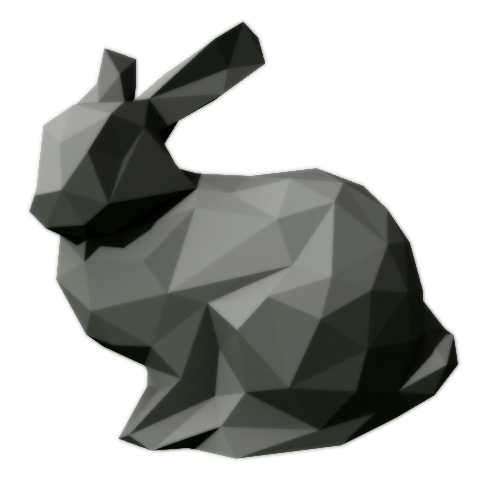
\includegraphics[height=1em]{figures/bunny-logo} \ \href{http://lgg.epfl.ch/}{LGG}'s course notes on remeshing, \textbf{Digital $3$D Geometry Processing}, given by B.Deng and B.Neubert in $2012$\\
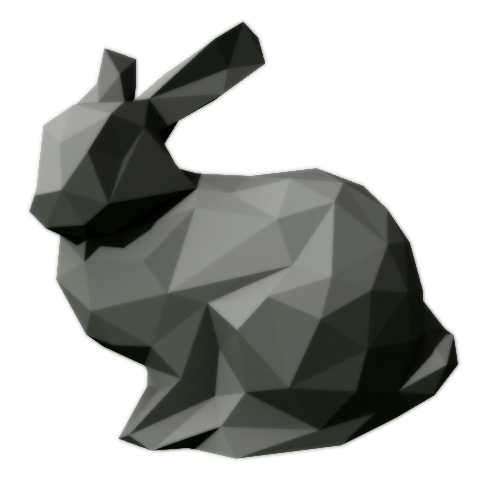
\includegraphics[height=1em]{figures/bunny-logo} \ Tutorials from \href{http://graphics.ethz.ch/publications/tutorials.php}{Computer Graphics Laboratory, ETH Zürich}\\
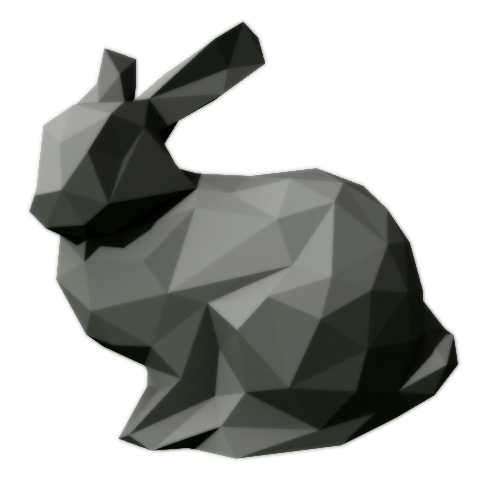
\includegraphics[height=1em]{figures/bunny-logo} \ Chapter $10$ (Remeshing) of \textbf{\href{http://graphics.ethz.ch/Downloads/Publications/Tutorials/2007/Bot07a/SIG07Notes.pdf}{Geometric Modeling Based on Polygonal Meshes}}, ACM SIGGRAPH 2007 Course Notes from M.Botsch et al.
}
\end{frame}


\end{document}